\documentclass[letterpaper,12pt,twoside=false,DIV=11]{scrartcl}

%----------------------CONFIG---------------------------
%math packages
\usepackage{amsmath,amssymb,amsthm,units,unitsdef}

%bibliography style and citation style, bibstyles to use: plainnat, abbrvnat, unsrtnat, named, chicago
%otherwise numerical citationstyle will be used
%\usepackage[authoryear,round]{natbib}

\usepackage{longtable,tabularx,tabulary,multirow,lscape}
\usepackage[font={sl},format=plain,labelfont=bf]{caption}

% colors
\usepackage{color,colortbl}
\usepackage[dvipsnames]{xcolor}
\definecolor{darkblue}{HTML}{00354C}

\usepackage{booktabs}
%\usepackage{showkeys} % shows the labels above the references for

%easier development
\usepackage{ifpdf}

\ifpdf
    \usepackage[pdftex]{graphicx}
    \usepackage[]{pdfpages} %for including full pdf pages
    \usepackage[pdftex,
        bookmarks,
        bookmarksopen=true,
        bookmarksnumbered=true,
        pdfauthor={Reto Trappitsch},
        pdftitle={On the origin of elements in the Milky Way - Homework},
        colorlinks,
        linkcolor=darkblue,
        citecolor=darkblue,
        filecolor=black,
        urlcolor=darkblue,
        anchorcolor=black,
        menucolor=black,
        breaklinks=true,
        pageanchor=true, %for jumping to a page
        plainpages=false,
        pdfpagelabels=true]{hyperref}
    \pdfcompresslevel=9
    \pdfoutput=1
    \DeclareGraphicsExtensions{.pdf,.png,.jpg,.jpeg}
\else
    \usepackage{graphicx}
\fi
\usepackage{rotating} % rotate figures
\usepackage{subcaption}
\usepackage{wrapfig}


\usepackage{fancyhdr}
\pagestyle{fancy}
%\addtolength{\headwidth}{\marginparsep} %these change header-rule width
%\addtolength{\headwidth}{\marginparwidth}
\lhead{}
\chead{\small\scshape On the Origin of Elements in the Milky Way} 
\rhead{} 
\lfoot{} 
\cfoot{\thepage} 
\rfoot{} 
\renewcommand{\headrulewidth}{.3pt} 
\renewcommand{\footrulewidth}{.3pt}

% Redefine author as topic
\newcommand{\topic}{\author}

%
%Redefining sections as problems
%
\makeatletter
\newenvironment{problem}{\@startsection
    {section}
    {1}
    {-.2em}
    {-3.5ex plus -1ex minus -.2ex}
    {2.3ex plus .2ex}
    {
        \pagebreak[3] % forces pagebreak when space is small; use \eject for better results
        \noindent\sffamily\bfseries Problem
    }
}
{
    %\vspace{1ex}\begin{center} \rule{0.3\linewidth}{.3pt}\end{center}}
    \begin{center}\large\bfseries\ldots\ldots\ldots\end{center}
}
\makeatother

% set enumerate to use letters
\renewcommand{\theenumi}{\alph{enumi}}

% newcommands
%============
% my short cuts
\providecommand{\e}[1]{\ensuremath{\times 10^{#1}}}
\providecommand{\ex}[1]{\ensuremath{^{#1}}}
\providecommand{\dex}[1]{\ensuremath{\delta^{#1}}}
\newcommand{\nean}{$^{22}$Ne($\alpha$,n)$^{25}$Mg}

% textnormal
\newcommand{\tn}{\textnormal}
% textregistered
\newcommand{\tr}{$^\tn{\textregistered}$}


%-------------------DOCUMENT---------------------------

\begin{document}


\title{Homework \#2}
\topic{Big Bang Nucleosynthesis, Stellar Evolution}
\date{Assigned: February 17, 2021 \qquad Due: March 1, 2021}

\maketitle
\thispagestyle{fancy}


\noindent\emph{Percentages for each problem of the total grade (100\%) as given. Sub-problems, if present, split the problem's percentage equally. Please show your work!}

\begin{problem}{Primordial versus Stellar Helium (20\%)}

We have seen that the \ex{4}He mass fraction made in the Big Bang was about 25\%. Let's investigate how much of the \ex{4}He in the Sun is still primordial. 

The Sun has a luminosity of $L_\odot = 3.8\times 10^{26}$\,W. This luminosity is sustained by constant hydrogen fusion to helium in the Sun's core. In the reaction $4\mathrm{H} \longrightarrow 4\mathrm{He} + \Delta E$, the energy released is 28.3\,MeV. Assuming that the current luminosity is valid for the whole lifetime of the Sun ($4.6\times 10^{9}$\,a) and that the total mass of the Sun is $M_\odot = 2\times 10^{30}$\,kg, calculate the total amount of \ex{4}He produced and express it as a mass fraction of the Sun's total mass. What does this tell you about the main source of \ex{4}He?

\end{problem}

\begin{problem}{Distances and redshifts (20\%)}

The Tadpole Galaxy (UGC 10214) is a barred spiral galaxy that has been disrupted by a collision with a smaller galaxy about 100 million years ago. Figure~\ref{fig:tadpole_galaxy} shows an image of the galaxy taken by the Hubble Space Telescope. 
The galaxy's velocity with respect to the Milky Way has been determined as 9401\,km\,s$^{-1}$. 
\begin{figure}[tb]
    \centering
    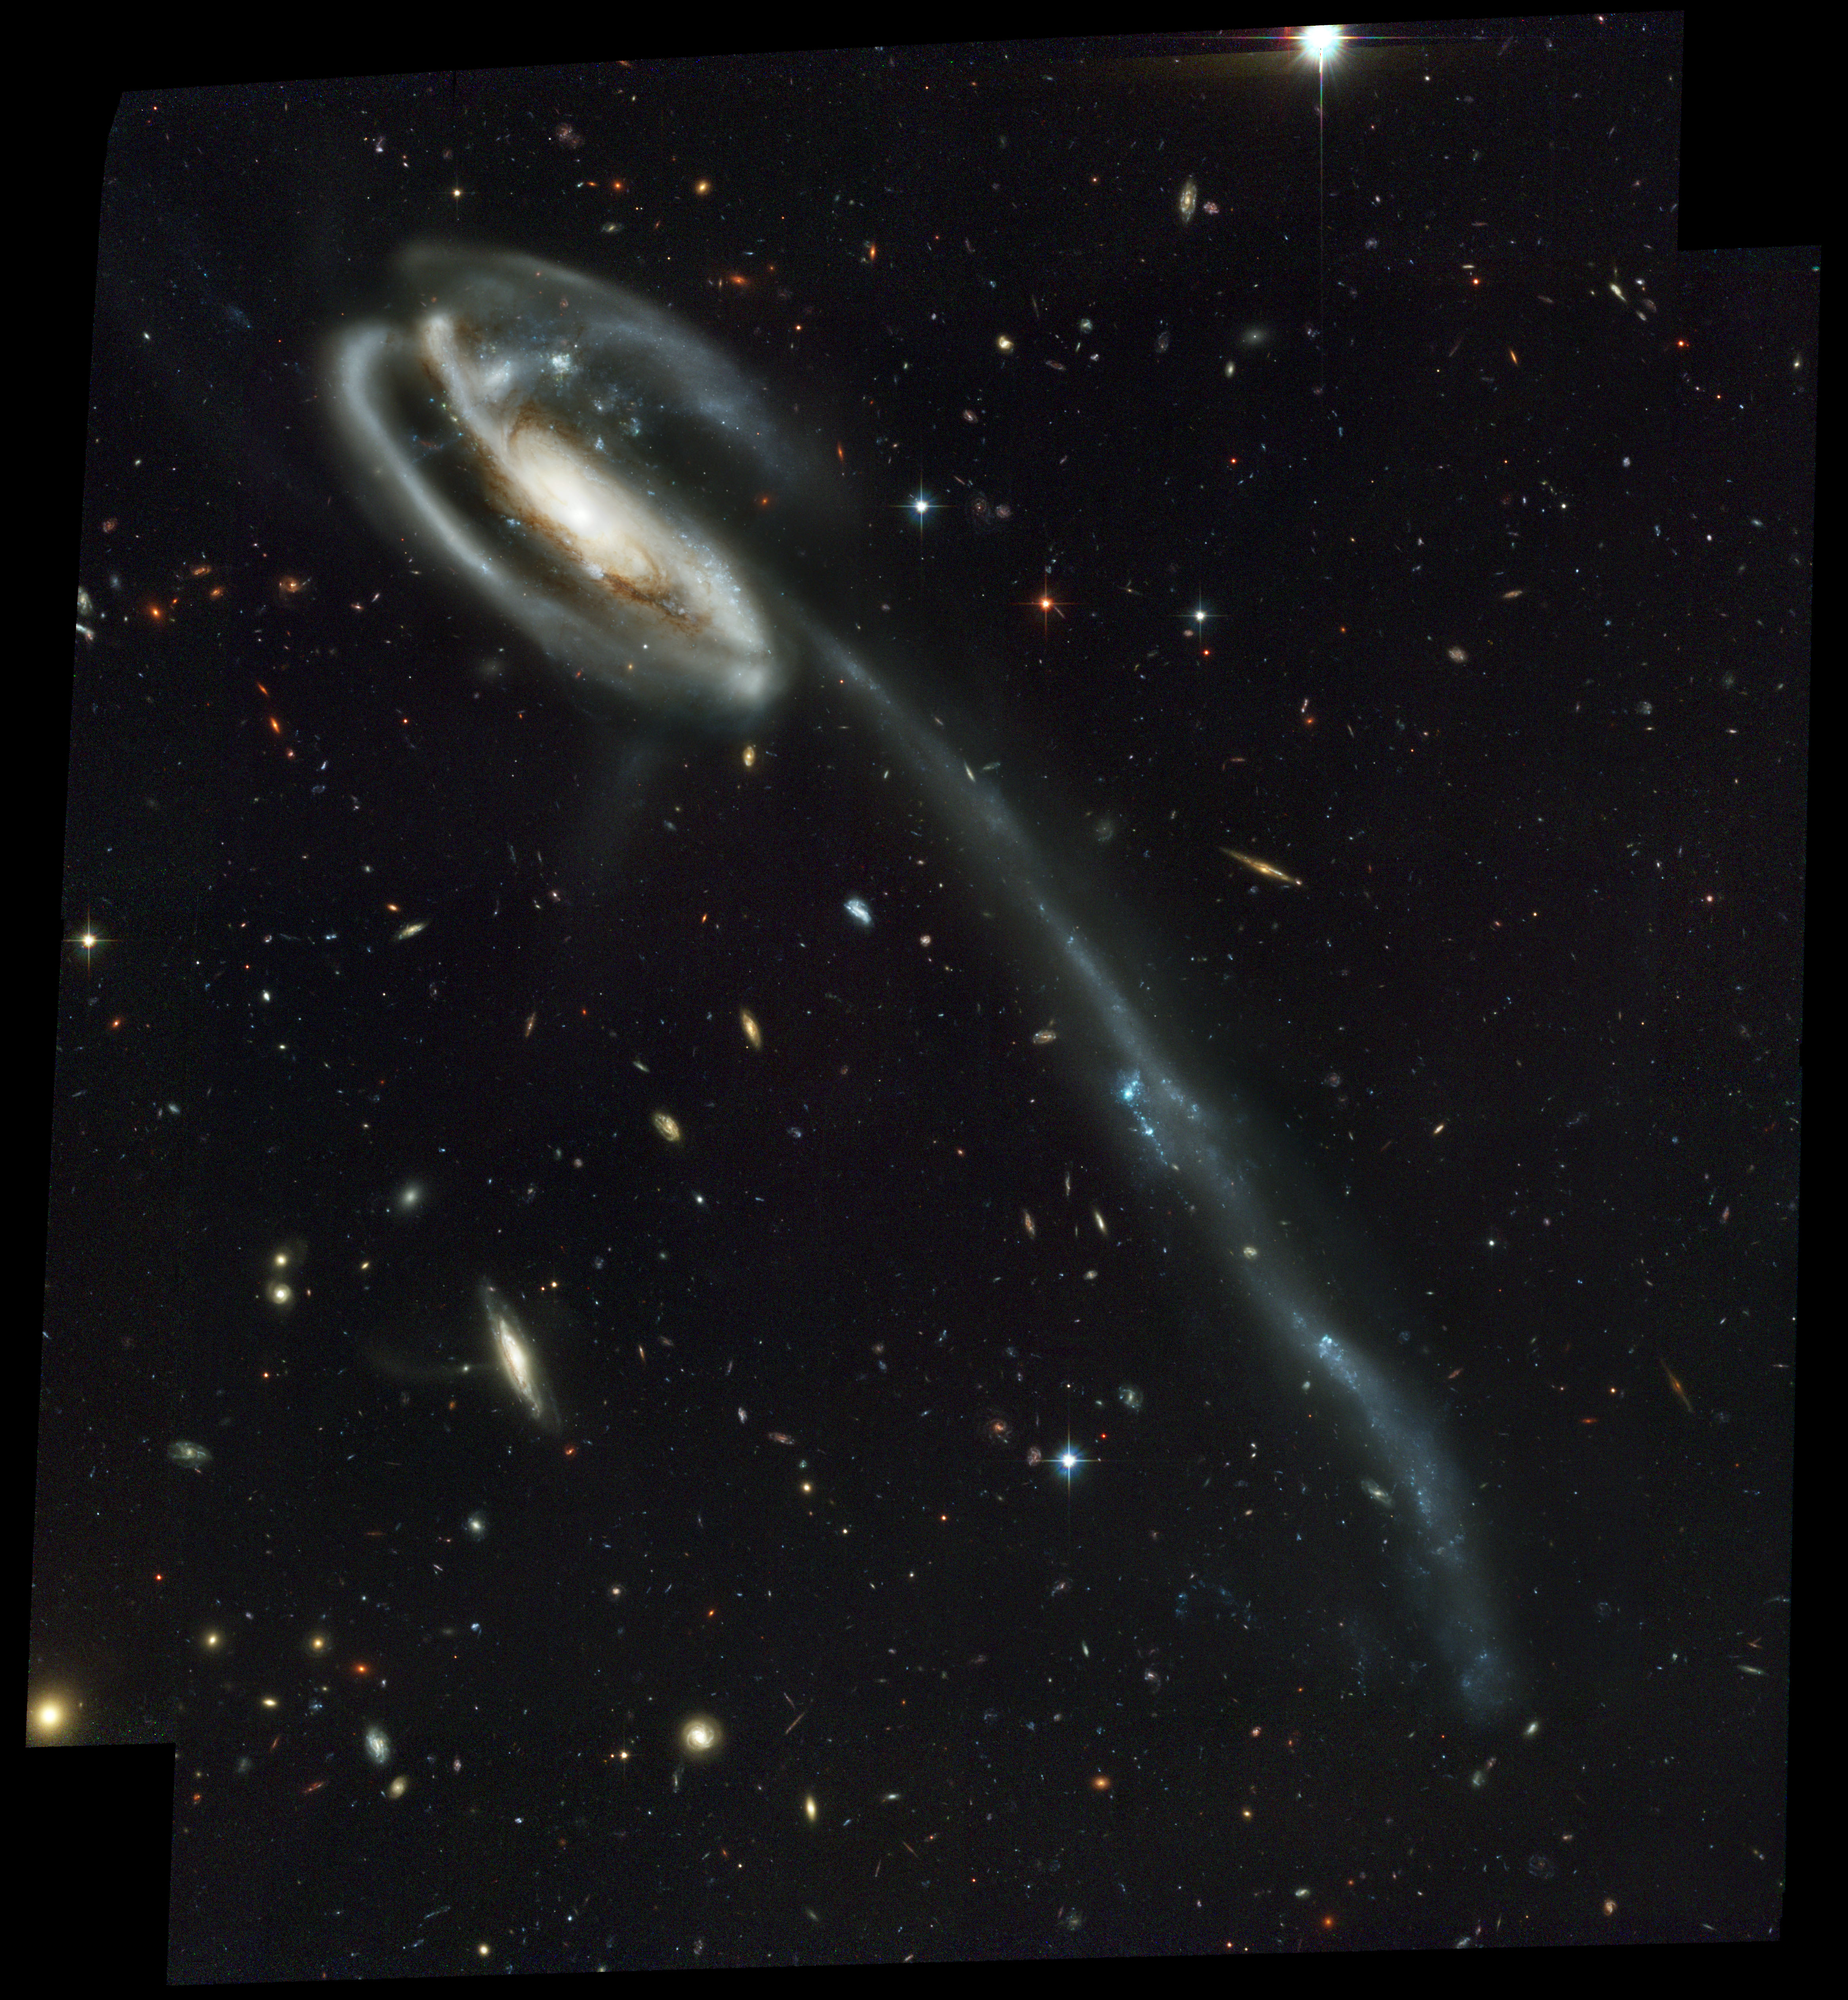
\includegraphics[width=0.5\textwidth]{tadpole_galaxy}
    \caption{Tadpole Galaxy imaged by the Hubble Space Telescope. Credit: NASA/HST.}
    \label{fig:tadpole_galaxy}
\end{figure}

\begin{enumerate}
    \item Assuming the Hubble constant $H_0 = 70\,\mathrm{km}\,\mathrm{s}^{-1}\,\mathrm{Mpc}^{-1}$, calculate the current distance from Earth to the Tadpole Galaxy in parsec (you can neglect the distance between the Earth's surface and the Hubble Space Telescope). What would the distance to this galaxy be in light years?
    \item Using the equation for the Doppler effect, determine the redshift $z$ under which we observe the Tadpole Galaxy.
\end{enumerate}

\end{problem}


\begin{problem}{Jeans Radius for the Solar System (20\%)} 
    We have discussed the Jeans mass, see equation~(3.8) of the lecture notes. If a molecular cloud exceeds the Jeans mass, it will collapse and lead to the formation of a star and, maybe some planets. Assuming that the Solar System started with a mass of $1\,M_\odot$, calculate the Jeans radius of the molecular cloud from which the Solar System formed. Assume a temperature of 10\,K for the molecular cloud and a composition of 75\% hydrogen and 25\% \ex{4}He. \emph{Note}: At this temperature, hydrogen should occur in the molecular form of H$_2$. Consider this when calculating the average mass $\mu$.
\end{problem}

\begin{problem}{Kepler's Third Law of Planetary Motion (20\%)}
    Kepler's third law states that the square of the orbital period $P$ divided by the cube of the distance from the Sun $R$ is constant for any body in the Solar System. Kepler's third law thus states:
    \begin{equation}
        \frac{T^{2}}{R^{3}} = \mathrm{constant}
    \end{equation}
    Show that this is true by deriving Kepler's third law using the virial theorem (equation (3.7) in the lecture notes) and explain what goes into the constant. \emph{Hint}: Kepler's third law is more or less derived in the lecture notes by setting the gravitational and centrifugal force equal. This derivation should help you when showing Kepler's third law using the virial theorem.
\end{problem}


\begin{problem}{The day(s) the Earth Stood Still (20\%)}
    The Earth orbits the Sun at a distance of 1\,AU with a period of 1 year. The gravitational and centrifugal force exactly compensate each other, thus keeping the Earth in orbit. Assume that all of a sudden the Earth stood still, i.e., the velocity would stop and the centrifugal force falls away. Calculate the time it would take for the Earth to crash into the Sun.
\end{problem}

\end{document}
